%%%%%%%%%%%%%%%%%%%%%%%%%%%%%%%%%%%%%%%%%%%%
%                                          %
% Important note on usage                  %
% -----------------------                  %
% This file must be compiled with PDFLaTeX %
% Using standard LaTeX will not work!      %
%                                          %
%%%%%%%%%%%%%%%%%%%%%%%%%%%%%%%%%%%%%%%%%%%%

\documentclass[3p,times]{elsarticle}
\usepackage{ecrc}
\usepackage{amsmath}
\usepackage{algorithm}
\usepackage{algpseudocode}
\usepackage[shortlabels]{enumitem}
\usepackage[flushleft]{threeparttable}
\volume{00}
\usepackage{booktabs}
\usepackage{multirow}
\firstpage{1}
\journalname{Journal of Public Economics}
\runauth{}
\usepackage{float}

%% The choice of journal logo is determined by the \jid and \jnltitlelogo commands.
%% A user-supplied logo with the name <\jid>logo.pdf will be inserted if present.
%% e.g. if \jid{yspmi} the system will look for a file yspmilogo.pdf
%% Otherwise the content of \jnltitlelogo will be set between horizontal lines as a default logo

%% Give the abbreviation of the Journal.
\jid{JPE}

%% Give a short journal name for the dummy logo (if needed)
\jnltitlelogo{Journal of Public Economics}
%% If using BibTeX, use the style file elsarticle-num.bst

%% End of ecrc-specific commands
%%%%%%%%%%%%%%%%%%%%%%%%%%%%%%%%%%%%%%%%%%%%%%%%%%%%%%%%%%%%%%%%%%%%%%%%%%

%% The amssymb package provides various useful mathematical symbols
\usepackage{amssymb}


%% The amsthm package provides extended theorem environments
%% \usepackage{amsthm}

%% The lineno packages adds line numbers. Start line numbering with
%% \begin{linenumbers}, end it with \end{linenumbers}. Or switch it on
%% for the whole article with \linenumbers after \end{frontmatter}.
%% \usepackage{lineno}

%% natbib.sty is loaded by default. However, natbib options can be
%% provided with \biboptions{...} command. Following options are
%% valid:

%%   round  -  round parentheses are used (default)
%%   square -  square brackets are used   [option]
%%   curly  -  curly braces are used      {option}
%%   angle  -  angle brackets are used    <option>
%%   semicolon  -  multiple citations separated by semi-colon
%%   colon  - same as semicolon, an earlier confusion
%%   comma  -  separated by comma
%%   numbers-  selects numerical citations
%%   super  -  numerical citations as superscripts
%%   sort   -  sorts multiple citations according to order in ref. list
%%   sort&compress   -  like sort, but also compresses numerical citations
%%   compress - compresses without sorting
%%
%% \biboptions{comma,round}

% \biboptions{}

% if you have landscape tables
\usepackage[figuresright]{rotating}
\usepackage{CJKutf8}
\usepackage{xcolor}
% put your own definitions here:
%   \newcommand{\cZ}{\cal{Z}}
%   \newtheorem{def}{Definition}[section]
%   ...

% add words to TeX's hyphenation exception list
%\hyphenation{author another created financial paper re-commend-ed Post-Script}

% declarations for front matter
\bibliographystyle{plainnat}
\begin{document}

\begin{frontmatter}

%% Title, authors and addresses

%% use the tnoteref command within \title for footnotes;
%% use the tnotetext command for the associated footnote;
%% use the fnref command within \author or \address for footnotes;
%% use the fntext command for the associated footnote;
%% use the corref command within \author for corresponding author footnotes;
%% use the cortext command for the associated footnote;
%% use the ead command for the email address,
%% and the form \ead[url] for the home page:
%%
% \title{Title\tnoteref{label1}}
% \tnotetext[label1]{asdfasdf}
\author{Chang Liu\fnref{label1}}
\author{Zhiwei Tian\corref{cor1}\fnref{label1}}
% \ead{tian.zhiwei@mail.shufe.edu.cn}
% \fntext[label1]{Shanghai university of finance and economics}
% \ead[url]{home page}
% \fntext[label2]{}
\cortext[cor1]{tian.zhiwei@mail.shufe.edu.cn}
% \address{Address\fnref{label3}}
% \fntext[label3]{}

\dochead{}
%% Use \dochead if there is an article header, e.g. \dochead{Short communication}

\title{What impact did China's value-added tax reform in 2019 have on the profitability of Chinese listed companies?}

%% use optional labels to link authors explicitly to addresses:
%% \author[label1,label2]{<author name>}
\address[label1]{Shanghai university of finance and economics}
%% \address[label2]{<address>}

\begin{abstract}
In the past decade, China's economy has shown a downward trend. To stimulate the economy and help companies in China survive better, in 2019, the Chinese government chose to implement a large-scale value-added tax reform. The reform mainly includes five aspects: lowering the VAT tax rate, giving additional input VAT deduction for certain industries, allowing excess input tax credits, expanding the scope of VAT deduction and increasing the VAT threshold. Based on the VAT invoice data from the China State Taxation Bureau and the operating data of Chinese listed companies, we examined 
what impact did the VAT reform have on the profitability of listed companies in China. Our findings show that when a company enjoys a higher effective VAT deduction rate in the reform, its profitability performance improves better. In addition, we find that its impact on the profitability of loss-making companies is much high than its impact on profitable companies even when their effective VAT deduction rate decreases by the same level, which  helps to explain why the value-added tax reform is more effective than the corporate income tax reform in helping companies survive.
\end{abstract}

\begin{keyword}
China's VAT Reform, Effective VAT Deduction Rate, Profitability Performance, Listed Companies 
\end{keyword}

\end{frontmatter}

%%
%% Start line numbering here if you want
%%
% \linenumbers

%% main text
\section{Introduction}
\label{intro}

Since the 21st century, China's total GDP has been showing a trend of increasing year by year. However, since 2010, the annual growth rate of China’s GDP has shown a downward trend. The growth rate of variable prices has dropped from $18.2\%$ in $2010$ to the lowest $7\%$ in 2015. Although GDP growth has rebounded in 2016, it dropped to $10.5\%$ again in $2018$ (Data from the National Bureau of Statistics, $2020$ update). The decline in economic growth has caused China's real economy to face severe challenges. Therefore, the Chinese government seeks to stimulate the economy through tax cuts to prevent a long-term economic downturn.

From ancient times to the present, different economists have been inconclusive on the issue of whether taxes should be increased or reduced in order to promote social and economic growth. Adam Smith and David Ricardo both believed that taxation has a hindering effect on economic growth. Also, According to the experimental results of \citet{levy2009behavioral}: an increase in the tax rate will arouse dissatisfaction among the people, who will punish tax collectors by reducing labor. However, Keynes believes that taxation is an important lever for regulating economic operations. During a recession, the government can use methods such as tax cuts and expansion of government expenditures to increase demand. Taxation methods can also be used to adjust income distribution, increase effective demand, and achieve stable macroeconomic growth.

Combining the experience of tax cut reforms in different countries in the past, many economists have explored the effects of tax cuts. Popular research perspectives include:

\begin{enumerate}[(1)]
    \item Macroeconomics: Many scholars believe that tax cuts are conducive to stimulating economic development ~\cite{lucas201214, garrison1992taxation}. However, ~\citet{giannitsarou2006supply} believes that tax cuts during the economic recession may not play a role in short-term fiscal stimulus, and only when the economy is booming, tax cuts will bring significant benefits.
    
    \item Labor supply: For example, ~\citet{eissa20081} explored the impact of the decline in the marginal tax rate of ETRA personal income tax in 1981 on the labor supply of married women, and the results showed that due to the decline in the marginal tax rate, the labor participation rate of high-income women increased from $47\%$ to $50\%$. ~\citet{kniesner2008evidence}, ~\citet{moore2002effects}, etc. also believe that after-tax wage increases from tax cuts can effectively stimulate labor supply and improve entrepreneurship. However, ~\citet{mankiw2006dynamic} added flexible labor supply, limited life, imperfect competition, and positive externalities of capital investment into the neoclassical growth model, pointing out that the increase in tax rate has adverse effects on labor and capital supply. 
    
    \item Savings accumulation: There are some controversies in the literature about the impact of tax reduction policies on savings and investment. In terms of savings, although lowering the marginal tax rate can increase the income available for savings and increase the after-tax income of savings, it will also bring an income effect that helps consumption. Therefore, the effect of tax cuts on savings is still not clear ~\cite{kniesner2008evidence}.
    
    \item Investment incentives: Most economists believe that tax cuts can incentivize investment. For example, ~\citet{liuhong2017} used panel data from 24 countries and found that higher corporate tax rates have a depressing effect on Japan's attracting overseas direct investment. ~\citet{chen2019tax} used China's 2009 data on value-added tax reforms aimed at reducing investment costs and found that the tax reduction policy has brought about $36\%$ investment growth. However, ~\citet{zee2002tax} believes that whether tax cuts promote corporate investment is uncertain, and the effect of tax reduction policies is mainly reflected in correcting market failures to make up for corporate investment costs. ~\citet{zhong2011value} also believe that the “VAT Transformation Reform” pilot program has no significant impact on corporate investment.
    
    \item Corporate performance: ~\citet{strulik2010anticipated} believe that corporate income tax relief policies can bring about $10\%$ increase in corporate income. {\color{red} ~\citet{yang2006addvalue}, ~\citet{wang2010Research}} believe that "VAT transformation reform" is conducive to improving corporate profitability, while {\color{red} ~\citet{liu2012Value}} believe that the reform has no significant impact on corporate performance. {\color{red}{~\citet{he2019can}}} used the data of Chinese enterprises and found that the value-added tax reduction has a greater effect on the entry of non-state-owned enterprises and small-scale enterprises, but it has no significant effect on the entry of state-owned enterprises and large-scale enterprises.
\end{enumerate}

\begin{figure}
    \centering
    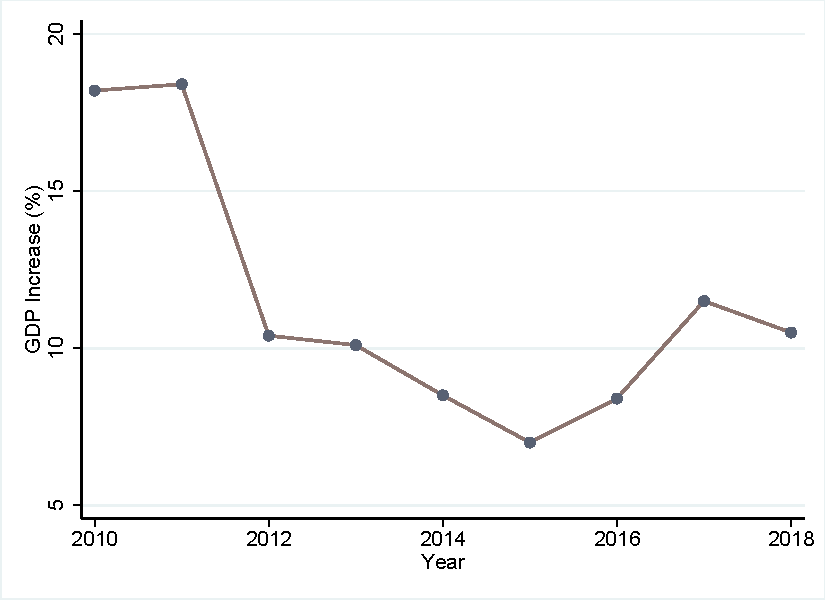
\includegraphics[width=0.7\textwidth]{1.pdf}
    \caption{\color{red}GDP}
    \label{fig:gdp}
\end{figure}
In China, since 2015, in order to stimulate the sustainable development of the Chinese economy, a wide range of applicable tax and fee reduction reforms have been implemented in China, including the reduction and exemption of various taxes such as personal income tax, corporate income tax, and value-added tax, as well as the suspension of various administrative fees. In 2015, at the initial stage of the implementation of the tax and fee reduction policies, the scale of tax and fee reduction was about $500$ billion RMB per year. By the end of 2018, this reform had reached the level of about $1300$ billion RMB.

However, with the rising status of value-added tax in China's tax system, as of 2018, value-added tax itself accounted for about $40\%$ of the total tax revenue in China. Therefore, starting in 2019, the Chinese government decided to implement a deeper and larger-scale tax reduction reform only for the value-added tax, which is the most important tax in China. This paper will focus on this “Value-added Tax Reform in 2019 ” as it is unprecedented, newly introduced and covers the entire country.

So far, the research on the tax reduction effect of VAT has mostly focused on the welfare effect ~\cite{blomquist2001tax, emran2005selective, whalley2005vat, carbonnier2007pays}, impacts on government revenue ~\cite{nichele1995simulation, jenkins2000vat, moore2015tax}, and changes in customer consumption ~\cite{blundell2009assessing, barrell2009economics}. In addition, some scholars have also explored the impact of the VAT reform on the micro-level enterprises. For example, ~\citet{shoup1969experience} and ~\citep{onji2009response} studied corporate response measures; ~\citet{fang2017asymmetric} explored the impact of VAT pilot expansion in 2012 on China's corporate total tax burden.

In the early stage of China's Value-added Tax Reform in 2019, there were many debates about whether to implement the value-added tax reduction reform or the corporate income tax reduction reform. 

Scholars such as {\color{red} Wan and Tang (2016)} build a micro-simulating model and find that further reductions in corporate income tax rates can effectively improve corporate operating performance and increase its profits, thereby indirectly promoting investment and employment. Moreover, the increase in corporate revenue is basically proportional to the decrease in corporate income tax rate.

However, more economists believe that the benefits of corporate income tax cuts can only be enjoyed by profitable companies, and cannot really reduce the tax burden of loss-making companies, especially start-ups. Therefore, we should choose to reduce the VAT rate as it is much more neutral compared to corporate income tax, let alone value-added tax is the most important source of tax revenue in China. More economists such as {\color{red} ~\citet{tang2020vatreduction} and ~\citet{yue2020empirical}} believe that the value-added tax reduction reform can better help enterprises reduce the pressure on survival and have more development opportunities.

Therefore, as China's 2019 VAT reform has just turned one year old, this paper decides to use tax data from the VAT reform and operational data from Chinese listed companies to explore whether the strategy chosen by the Chinese government to reduce VAT helps to alleviate the pressure on list companies and effectively helps them to improve their profitability performance.


\section{Policy background}\label{sec:2}
In the past decade, China's economy has shown a downward trend as a whole. The growth rate of gross national product has decreased year by year, market demand has been weak, export growth has slowed, demographic dividends have decreased, and labor costs have risen. At the same time, there are constant calls from the private sector regarding the excessive tax burden of enterprises and the urgent need for tax cuts. Taxation is an important lever to regulate economic operation. During the period of cyclical economic downturn, the government can increase effective demand through tax cuts, expand government expenditures, and use taxation to regulate income distribution to achieve stable macroeconomic growth.

As mentioned before, the value-added tax has been China's largest tax source in recent years. Before the reform in 2018, value-added tax revenue accounted for $39.3\%$ of total tax revenue. In comparison, corporate and personal income tax only accounted for $22.6\%$ and $8.9\%$, respectively (National Bureau of Statistics of China, 2018). 

Before the 2019 VAT reform, China’s value-added tax rate was relatively high: $16\%$ for general commodities. Moreover, there were three different rates for different goods and services, and the difference between the highest rate of $16\%$ and the lowest rate of $6\%$ was as high as $10\%$, which was not in line with the tax neutrality of VAT and the regulatory role of VAT was not fully utilized. 

Therefore, in 2019, the Chinese government chose to implement a large-scale value-added tax reform, and hopes to gradually reduce the difference in the value-added tax rate between different goods and services, until the tax rate consolidation is realized in the future.

China's value-added tax reform in 2019 is one of the largest tax reduction reforms in history, and this reform not only reduces the tax rate, but also includes a number of adjustments to value-added tax related policies, mainly including the following five aspects:

\begin{enumerate}[(1)]
    \item Lowering the VAT tax rate: Prior to the reform, China's VAT rate was divided into three bands, with $16\%$ applied to most sales and imports, $10\%$ applied to a small number of commodity categories such as agricultural products and energy production, and $6\%$ applied to services revenue. Then in the 2019 reform, the original $16\%$ VAT rate was adjusted to the current $13\%$, and the $10\%$ VAT rate was adjusted to the current $9\%$. Moreover, the changes in tax rate will not only affect the companies that originally applied the $16\%$ and $10\%$ tax rates, but also affect the companies that originally applied the $6\%$ tax rate by affecting the input tax on the value-added tax amount.
    
    \item Allowing additional input VAT deduction for service industries: After the 2019 VAT reform, taxpayers in the production service industry and life service industry can add an additional $10\%$ or $15\%$ as a deduction to the original deductible input tax base, thereby reducing the final taxable amount.
    
    \item Allowing excess input tax credits: As loss-making companies and new start-ups are more likely to generate value-added tax refunds, compared with other tax reduction and fee reduction policies, the taxation refunding for value-added tax policies can not only reduce the tax burden of enterprises, but also, it can help loss-making companies turn losses into profits and reduce the initial investment costs of enterprises, thereby encouraging innovation and entrepreneurship.
    
    \item Expansion of the scope of deduction: In 2019 VAT reform, for the first time, passenger transportation-related services, such as transportation costs incurred by corporate employees on business trips, are included in the scope of input VAT deductions. In which way, the value-added tax becomes more neutral, and further reduces the tax burden of enterprises.
    
    \item Increasing the tax threshold: The value-added tax threshold for small-scale taxpayers has been raised from $30000$ RMB to $100000$ RMB, which significantly reduced the tax burden for enterprises with original sales between $30000$ RMB and $100000$ RMB.
    
\end{enumerate}

\begin{figure}
    \centering
    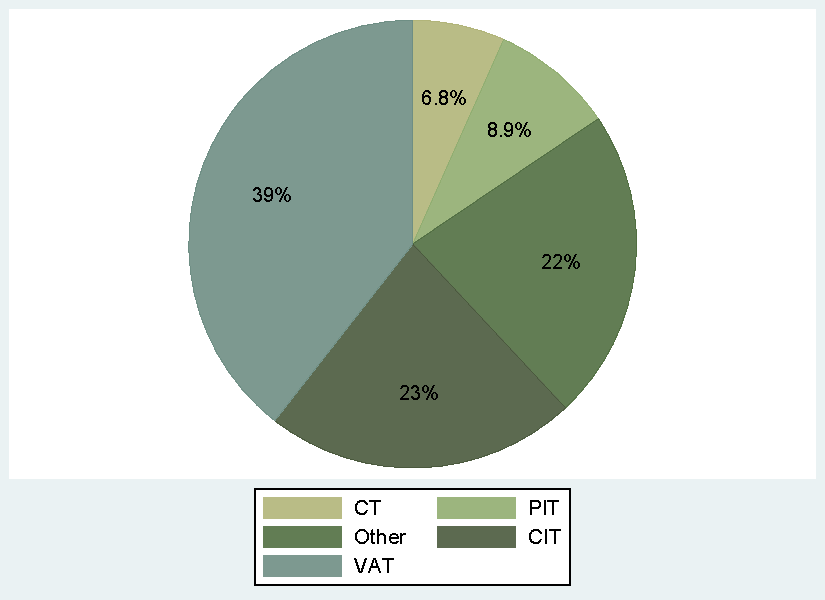
\includegraphics[width=0.7\textwidth]{2.pdf}
    \caption{Caption}
    \label{fig:index}
\end{figure}
In early 2020, by analyzing the invoice data of different industries in China, we find that although the magnitude of tax reduction varies from low to high for different industries, the VAT tax burden of each industry is  decreasing, which is in line with expectations. The difference in the rate of tax reduction among different industries is mainly due to the adoption of differentiated tax reduction policies for goods and services previously subject to different VAT rates.

In this paper, we decide to use the VAT invoice data in the system of Chinese tax authorities to calculate the “effective VAT reduction rate” under the 2019 China VAT tax reform, and here are steps on how we calculate the“Effective VAT Reduction Rate” $r_i$:

\begin{algorithm}[htp!]
\caption{{\color{red} Calculate the Effective VAT Reduction Rate}}
\begin{algorithmic}[1]
\State Select industries $I_i$ as the classification criteria to obtain invoice data for all operations  $O_i$ in 2019 for each industry
\begin{equation*}
    I_{i} = Industry\_I\_of\_Company\_ i,\quad O_{i} = All\_Business\_ Operations\_of\_Industry\_i 
\end{equation*}
\State Calculate the VAT $T_{i,\, old}$ the industry would have paid for all its operations happened in 2019 if the old VAT policy prior to the 2019 reform had been applied and the VAT $T_{i,\, new}$ the industry actually paid for all its operations happened in 2019 with the new VAT policy after the 2019 VAT reform.
\begin{equation*}
    T_{i,\, old} = VAT\_Rate_{i,\,2018}*O_{i,\, 2019}
\end{equation*}
\begin{equation*}
    T_{i,\, new} = VAT\_Rate_{i,\,2019}*O_{i,\, 2019}
\end{equation*}
\State Compare the difference $R_i$ between the VAT payable before and after the reform.
\begin{equation*}
    R_i = T_{i,\, old} - T_{i,\, new}
\end{equation*}
\State Use the tax saving amount $R_i$ to calculate the “Effective VAT Reduction Rate” $r_i$ by dividing it with the amount of VAT invoiced revenue actually incurred by each industry in 2019.
\begin{equation*}
    r_i = R_i / Invoice_{i,\,2019}
\end{equation*}
\end{algorithmic}\label{VAT_reduction_rate}
\end{algorithm}

Overall, by the implementation of the VAT reform in 2019, China has collected less VAT taxes by a total of $860.9$ billion RMB, and the average VAT reduction rate for the entire country is $16.13\%$. In detail, the tax reduction rate was higher in the wholesale and retail industry as well as the manufacturing industry than other industries. 

\section{Theoretical Analysis and Hypothesis}
\subsection{Theoretical Analysis}
For a long period of time before, due to the "easy transfer" of the VAT burden in the traditional sense, it is generally believed that changes in the VAT rate will not have a significant impact on enterprises (documentation). However, in the past two decades, with the continuous deepening of related theoretical and empirical research, more and more evidences show that the value-added tax rate does affect the status and behavior of enterprises. From the perspective of the influence mechanism, this article believes that the "price effect" and the "tax burden effect" are important ways to realize the impact of the adjustment of the value-added tax rate on the overall profit rate of the enterprise and the living space.

\subsubsection{Price effect}
"Price effect" is the mainstream argument in the existing literature to analyze the relationship between the value-added tax rate and the value of the enterprise, mainly focusing on the transfer mechanism of the value-added tax burden. Although value-added tax is an indirect tax and its tax burden can be completely passed on to the final consumer under ideal conditions, in the actual market environment, the value-added tax burden can often only be partially passed on. Constrained by the price elasticity of demand for services. This effect is the "price effect" of the value-added tax rate affecting the value of the enterprise~\cite{liu2018theimpact}.

Specifically, in the real market environment, the price elasticity of demand will hardly be completely elastic or completely inelastic. In this case, the introduction of value-added tax will increase the actual purchase price of goods or services, thereby making consumers The demand for goods or services has declined. At this time, companies usually choose to lower prices appropriately in response to reduced demand. Therefore, downward shifting of demand and prices will reduce producer surplus. In other words, companies must bear part of the value-added tax burden themselves, and the greater the price elasticity of the demand for goods or services provided by the company, the less value-added tax burden the company will pass on to consumers, because the company itself bears the value-added tax burden. And the greater the loss to corporate value.

Therefore, the reduction of the value-added tax rate can increase the profit margin of the company by reducing the loss caused by the value-added tax burden that cannot be passed on by the company. Larger, the more obvious this lifting effect.

\subsubsection{Tax burden effect}
Different from the "price effect" related to the price elasticity of demand, the "tax burden effect" does not involve the mechanism of value-added tax burden transfer, but from the perspectives of business operations and accounting practices, considering the so-called value-added tax actually borne by the enterprise. "Additional tax burden" mainly includes the following four aspects:
\begin{enumerate}[(1)]
    \item The value-added tax cannot be deducted when the input value-added tax is deemed to be sold or the invoice is not obtained as required. The company needs to bear this part of the value-added tax burden{\color{red}~\cite{liu2018theimpact}}.
    \item Due to the Chinese market In transactions, tax-included prices are often used for settlement. In the event of bad debt losses, the corresponding VAT output tax will not be available, which will increase the corporate tax burden{\color{red}~\cite{yue2020empirical}}.
    \item In cases such as credit sales, the company actually needs to advance the value-added output tax, so as to bear the corresponding time cost and opportunity cost{\color{red}~\cite{lv2008Improvement}}.
    \item The urban maintenance and construction tax and educational surcharges directly related to the value-added tax are also components of the “extra tax burden” of the value-added tax.
\end{enumerate}
When the value-added tax rate is lowered, the "extra tax burden" of value-added tax arising from the above-mentioned deemed sales, bad debt losses, and credit sales in the actual operation of the company will be reduced accordingly, and the reduction of tax burden and time cost will be reduced. It is beneficial to increase the operating profit margin of the enterprise and improve the living space.

\subsection{Hypothesis}
Based on the above relevant analysis of "price effect" and "tax burden effect", this article proposes the following hypotheses:
\begin{enumerate}[label={\textbf{H\arabic*}:}]
    \item The adjustment of the value-added tax rate will significantly affect the profit margin of the enterprise. When the value-added tax rate is lowered, corporate profits will be significantly improved.
    \item The adjustment of the value-added tax rate will significantly affect loss-making enterprises. When the value-added tax rate is lowered, it can increase the probability of loss-making companies turning losses into profits.
    \item The effect of the adjustment of the value-added tax rate on the profitability of enterprises is more obvious in enterprises with high price elasticity of demand and high value-added tax "extra tax burden".
\end{enumerate}

\section{Data and Methodology}
\subsection{Empirical Strategy}
The 2019 value-added tax reform can reduce corporate value-added tax and urban construction tax-related costs, and help Chinese companies effectively increase their after-tax profits. Especially for some companies with negative net profits, deepening the reform of value-added tax can help companies with poor operating performance to reduce the burden, improve their living space, and help them turn losses into profits as soon as possible.

This paper decides to choose a panel data fixed-effect regression model similar to the DID model for empirical exploration. The 2019 value-added tax reduction reform has high universality due to its many tax reduction rules, so that this reform basically covers all Chinese enterprises. Therefore, the traditional DID model is not suitable due to the lack of accurate control groups. As the empirical research choice of this article.

In the DID-like model selected in this paper, the core explanatory variable is the intersection of the average value-added tax reduction rate of each industry and the time dummy variable. In order to fully consider the heterogeneity among regions, industries, and quarters, the fixed effects absorbed in the model include: the listed company itself, the registered address of the listed company, the quarter, and the 20 industry category codes to which the listed company belongs. The overall regression model formula is as follows:
\begin{equation}
    y_{i,\,t} = \beta_0 + \beta_1 r_i D_i + \beta_2 X_{i,\,t} + v_i + \epsilon_{i,\,t}
\end{equation}
where $i$ and $t$ respectively represent the individual and period of the corresponding listed company; $r_i$ is the actual average tax reduction rate of various industries in the deepening of the value-added tax reform, $D_i$ is the time dummy variable, and the value is set to 1 in 2019 and after, $v_i$ It is the quarterly heterogeneity of different registered provinces, different industry categories, and the company's own heterogeneous absorption. $\epsilon_{i,\,t}$ is the random disturbance term of this type of DID fixed-effect model; $X$ is the multiple sets of control variables mentioned above.

\subsection{Data and variables}
First, in order to verify the above hypothesis 1 and 2, the explained variables selected in this paper are: the profit rate of the enterprise and whether the dummy variable is profitable.

Secondly, in the part of explanatory variables, unlike most of the current literature (specific literature) that uses corporate tax burden change rate to reflect the degree of tax reduction, this article decides to directly select deepening value-added tax according to the reformed value-added tax reduction rate of each industry Is an explanatory variable. The main reasons are as follows: First, the tax reduction rate of the value-added tax industry is directly selected as an explanatory variable, and the impact of other tax reduction preferential policies on Chinese listed companies can be stripped; second, because the usual changes in corporate value-added tax burdens are not affected by tax reduction policies The impact is also affected by the changes in the company’s own sales composition. Different goods and services in China may correspond to different VAT rates. Therefore, when the company’s sales of goods and services change, the company’s overall VAT burden rate will also change. If there is a change, then the change in the corporate tax rate is likely not caused by the tax reduction policy. 

Therefore, this paper decides to select the VAT industry tax reduction rate $r_i$ disclosed in the research report commissioned by the State Administration of Taxation by Shanghai University of Finance and Economics instead of the overall VAT burden change as an explanatory variable to more fully and accurately reflect the direct impact of tax reduction on enterprises. The specific calculation formula of the tax reduction rate is in {\color{red} Chapter 2\ref{sec:2}}.

It is worth noting that the amount of tax reduction is based on the amount of value-added tax after the deepening of the value-added tax reform corresponding to the amount of invoices actually generated by the enterprise and the assumptions are based on the original value-added tax rate, the original additional deduction policy, the original deduction scope, and the original retained credit. The tax rebate policy and the difference in the amount calculated by the combined effect of the original levy point is calculated, which is the total of the five parts of the tax reduction benefits that the enterprise really enjoys this deepening of the value-added reform reform. It is not just the tax reduction brought about by the decline in the tax rate.

In addition, because the invoice data of listed companies can only be obtained from the tax system, data confidentiality restrictions prevent the tax reduction rate of each company from being disclosed. Therefore, we decided to use the average tax reduction rate of the company's industry as the tax reduction rate in the explanatory variable in the model. According to the 2017 National Economic Industry Classification (GB/T 4754-2017) issued by the Chinese government, all industries in my country are divided into 97 categories. Therefore, this article selects the calculated average value-added tax of these 97 categories The tax reduction rate matches each listed company, that is, the tax reduction rate of the industry category to which each listed company belongs is used as the estimate of each company's own explanatory variable. In addition, these 97 categories are further summarized into 20 broader industry categories in the (GB/T 4754-2017) standard. We disclosed the average tax reduction rates of the 20 industry categories of these 97 industries as a reference.

After calculating the value-added tax reduction rate based on the above logic, the tax reduction rate is multiplied by the time dummy variable to make the explanatory variable in the text genre DID model. Therefore, the time dummy variable $D_i$ needs to be set in the explanatory variable, which should be set before 2019. The time dummy variable is set to 0; after the formal implementation of the deepening of the value-added tax reform in 2019, the time dummy variable is set to 1.

Finally, the control variables selected in this article mainly cover three aspects of the nature of the enterprise: profitability, operating ability and solvency. This article selects four financial management indicators from these three aspects for analysis and control. This is because for every enterprise, at every stage of development, there will be more plans and goals in the operation process, such as controlling the total amount of liquidity, controlling the asset-liability ratio, controlling the turnover rate, etc., so choose here The multi-index approach corresponds to more absolute values. It comprehensively evaluates the development status of the enterprise from multiple dimensions. It is also a relatively comprehensive control variable, which more completely and accurately reflects the truest operating level of the enterprise. Earnings per share indicators control equity changes from the perspective of owner’s equity and measure the strength of corporate profitability; total asset turnover can reflect the company’s operating efficiency to reflect the company’s current status and activity; asset-liability ratio and solvency It is also one of the important measures of corporate viability. In addition, since the deepening of the value-added tax reform will also affect government fiscal expenditures and indirectly affect the government subsidies of listed companies in my country, in the model, the amount of government fiscal subsidies received by enterprises is added as a control variable.
\newcommand{\tabincell}[2]{\begin{tabular}{@{}#1@{}}#2\end{tabular}}
\begin{table}[htp!]
% \setlength{\abovecaptionskip}{0.5cm}
% \setlength{\belowcaptionskip}{0.5cm}
\begin{center}  
    \caption{Explanations Of Control variables}
    \begin{tabular}{c|c|c}
         \toprule\toprule
         Evaluation Dimension & Financial Indicator & Calculation Caliber\\
         \hline
         Operating Capacity & Turnover Rate of Total Assets (TAT) & Operating income / Total Assets\\
         \hline
         \multirow{4}{*}{Solvency}& Debt Asset ratio (DAR)&Total liabilities / Total assets \\\cline{2-3}&Acid Test Ratio (ATR)&\tabincell{c}{(Cash and Cash Equivalents\\+Held for Trading Financial Assets\\+Accounts Receivable)/Current Liabilities}\\
         \hline
         Political Influence&Government Grants Amount (GGA)&Amount of Government financial Grants\\
         \bottomrule
    \end{tabular}
    \label{tab:control_var}
\end{center}   
\end{table}
According to the above settings, in order to verify Hypothesis \textbf{H1} and Hypothesis \textbf{H2}, the specific empirical test model is as follows:
\begin{equation}
    \begin{split}
        ProfitRate_{i, \, t} = \beta_0 + \beta_1 r_{i} D_i + \beta_2 X_{i, \, t} + v_i + \epsilon_{i,\,t}\\
        IsProfit_{i, \, t} = \beta_0 + \beta_1 r_{i} D_i + \beta_2 X_{i, \, t} + v_i + \epsilon_{i,\,t}
    \end{split}
\end{equation}
where $X_{i, \, t}\in\left\{EPS_{i, \, t},TAT_{i, \, t},DAR_{i, \, t},ATR_{i, \, t},Gov\_Grant_{i, \, t}\right\}$.

The data related to business operations in this article are mainly derived from the annual report data of 3367 companies listed in China in 2017-2019 of the Guotaian CSMAR database and Wind database. After excluding outliers and severely missing data, there are a total of $8547$ items, including basic information and revenue of listed companies. Status, profit status, R\&D investment, asset investment, number of employees, government subsidies and other relevant data. In addition, the tax reduction rate data for the 2019 deepening of the value-added tax reform in various industries comes from the industry average tax reduction rate calculated by the Shanghai University of Finance and Economics Public Policy and Governance Institute through the State Administration of Taxation VAT invoice data, including the tax reduction rate by industry category and industry category.
\begin{table}[htp!]
\caption{Descriptive Statistics of Variables}
    \centering
    \begin{tabular}{c|c|c|c|c|c|c}
    \toprule\toprule
        Category & Varibale & Observation & Mean & Std.Dev. & Min & Max\\
         \hline
        \multirow{2}{*}{Dep.Var.} & Profit Rate (\%) & 8547 &	1.5	&56.3&	-1131.2	&66.5 \\\cline{2-7}&IsProfit (Dummy.Var.)&8547&	0.8	&0.4&	0&	1\\
        \hline
        {Indep.Var.} & Effective VAT Reduction Rate & 8547	 & 0.192 & 	0.059 & 	-0.032 & 	0.359\\
        \hline
        \multirow{4}{*}{Control.Var.} & TAT (\%) &8547	&60.3&	37.7&	2.2&	242 \\\cline{2-7}&DAR (\%)&8547&	41.3	&20.1&	6.2&	97.2	1\\\cline{2-7}&ATR (\%)&8547&197.8&	203.3&	18.6	&1316.1	1\\\cline{2-7}&GGA (RMB 100M)&8547&0.6	&2.8&	0&	112.7\\
    \bottomrule
    \end{tabular}
    \label{tab:Descriptive_stat}
\end{table}

\begin{figure}
    \centering
    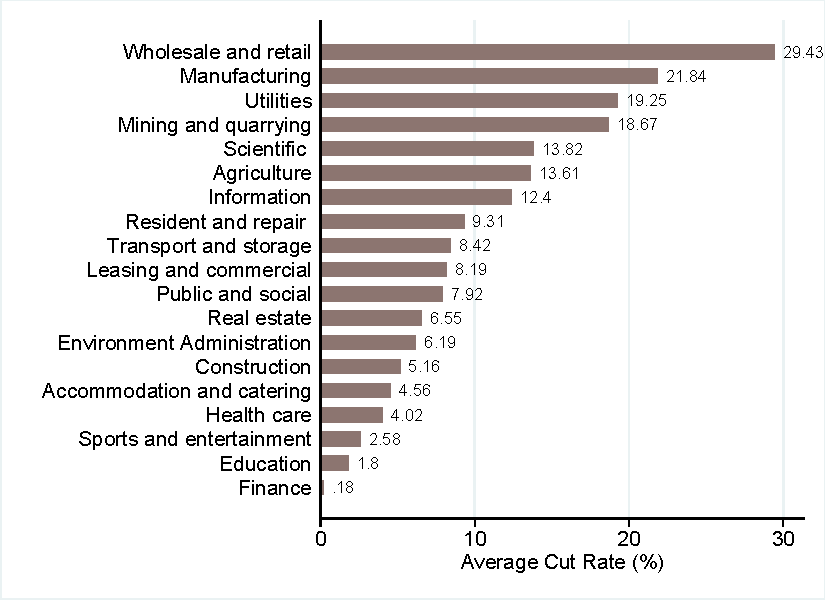
\includegraphics[width=0.7\textwidth]{3.pdf}
    \caption{Caption}
    \label{fig:my_label}
\end{figure}

\section{Empirical Results}
\subsection{Impact on Enterprise Profitability}
This chapter uses the DID-like fixed-effects panel model to conduct empirical regression analysis. In order to make the results more robust and credible, this article decides to use the method of gradually adding each control variable in the process of specific empirical analysis. Models (1) to (6) gradually add control variables EPS, total asset turnover ratio TAT, asset-liability ratio DAR quick ratio ATR, and government financial subsidies Ln\_Gov\_Grants. Among them, the explanatory variable in the model is the company’s annual operating profit rate ProfitRate, which is calculated by dividing the company’s annual operating profit by the company’s operating income. The explanatory variable is the value-added tax industry average tax reduction rate and the time dummy variable. The multiplication item $r_i D_i$, $D_i$ is a time dummy variable. In 2019, it is 1 due to the implementation of the deepening of the VAT reform. The value of this variable is 0 in 2018 and previous years. In addition, in order to further improve the accuracy of the model and absorb more heterogeneity, the following table also performs fixed-effect absorption on the information of listed companies in my country, the information on the registration place, and the industry category information to which they belong. At the same time, a robust standard error method after clustering adjustment is adopted for heteroscedasticity.

According to the results in table \ref{tab:esti_prof}, in models (1) to (6), the results of the explanatory variable $r_i D_i$ correlation coefficient are always significantly positive, indicating that in the deepening of the value-added tax reform, as the tax reduction rate increases, my country’s listed companies The profit margin has also been significantly improved.



It is worth noting that, according to relevant research and analysis, one of the important reasons for my country to further deepen the value-added tax reform in 2019 also includes important assistance to relevant loss-making enterprises to further reduce the tax burden, enhance the vitality of the enterprise, and win the living space. Since the scope of the preferential corporate income tax reduction and exemption is mainly related to profitable enterprises, the loss-making enterprises cannot enjoy the preferential corporate income tax-related preferential policies. Therefore, in order to further quantify the impact of the tax reduction rate of the value-added tax reform on the operating profits of some loss-making companies of my country's listed companies.

\begin{table}[htp!]
    \centering
    \caption{Regression of Effective VAT Reduction Rate on Profit Rate}
    \begin{threeparttable}
    \begin{tabular}{l|ccccc}%\\ 
        \toprule\toprule
        &\multicolumn{5}{c}{Dependent Variable: Profit Rate}\\
        \cline{2-6}
         & (1) & (2) & (3) & (4) & (5) \\
         \hline
         &  &  &  &  &  \\
        EVRR&0.10\tnote{**}&	0.24\tnote{***}	&0.23\tnote{***}&	0.19\tnote{***}	&0.11\tnote{***}\\&
        (0.04)&	(0.04)&	(0.04)	&(0.05)&	(0.04)\\
        TAT&&0.32\tnote{***}&	0.27\tnote{***}	&0.26\tnote{***}&	0.25\tnote{***}\\&&
        (0.08)&	(0.08)	&(0.08)	&(0.08)\\
        DAR&&&-1.21\tnote{***}&	-1.31\tnote{***}&	-1.31\tnote{***}\\&&&
        (0.32)&	(0.36)&	(0.36)\\
        ATR&&&&-0.02\tnote{*}&	-0.02\tnote{*}\\
        &&&&(0.01)&	(0.01)\\
        GGA&&&&&0.03\\
        &&&&&(0.02)
        \\
          &  &  &  &  &  \\
        ID FE & Yes & Yes& Yes& Yes& Yes  \\
        Address FE & Yes & Yes& Yes& Yes& Yes \\
        Quarter $\times$ Industry FE & Yes & Yes& Yes& Yes& Yes  \\
         &  &  &  &  &  \\
        
        Observations  & 8,239 & 	8,239	 & 8,239 & 	8,239 & 	8,239 \\
        R-squared & 0.581&	0.584&	0.601&	0.601	&0.602 \\
        \bottomrule
    \end{tabular}
    \begin{tablenotes}
        \item $^{***}$, $^{**}$, $^{*}$ indicate significant at the level of $1\%$, $5\%$ and $10\%$, respectively.
    \end{tablenotes}
    \end{threeparttable}
    \label{tab:esti_prof}
\end{table}


According to the results in Table \ref{tab:esti_loss}, it can be found that when companies with a positive operating profit rate in a certain year are excluded, when only a part of the loss-making enterprises are empirically analyzed, in model (6), the correlation coefficient relationship between the operating profit rate and the tax rate is $1.32$, which is significantly greater than $0.24$ in the analysis of all companies in the previous table. Therefore, we can find that the deepening of the value-added tax reform in 2019 has a more significant and strong driving effect on these $978$ loss-making companies. The value-added tax reform has boosted the operating profit rate of $978$ loss-making companies about five times the average boost effect of the $3367$ listed companies in my country in the sample. This model further demonstrates that the deepening of the value-added tax reform improves the survival of enterprises. Space, the original intention and effect of reforms to enhance the vitality of the real economy.

\begin{table}[htp!]
    \centering
  \caption{Regression of Effective VAT Reduction Rate on Profit Rate of Loss-Making Companies}
    %\resizebox{\linewidth}{!}{%
    \begin{tabular}{l|ccccc}%&\\ 
    \toprule\toprule
    &\multicolumn{5}{c}{Dependent Variable: Profit Rate of Loss-Making Comapnies}\\
\cline{2-6}
 & (1) & (2) & (3) & (4) & (5) \\
 \hline
 &  &  &  &  &  \\
EVRR&1.00\tnote{***}&	1.08\tnote{***}&	1.38\tnote{***}&	1.40\tnote{***}&	1.37\tnote{***}\\&
(0.33)&	(0.32)&	(0.33)&	(0.34)&	(0.35)\\

TAT&&0.80\tnote{***}&	0.73\tnote{***}&	0.74\tnote{***}&	0.73\tnote{***}\\&&
(0.25)&	(0.24)	&(0.24)&	(0.24)
\\
DAR&&&-1.90\tnote{*}&	-1.99\tnote{*}&	-1.92\tnote{*}\\&&&
(0.99)&	(1.08)&	(1.04)\\
ATR&&&&-0.03&	-0.02\\
&&&&(0.05)&	(0.05)\\
GGA&&&&&0.06\\
&&&&&(0.05)
\\
  &  &  &  &  &  \\
ID FE & Yes & Yes& Yes& Yes& Yes  \\
Address FE & Yes & Yes& Yes& Yes& Yes \\
Quarter $\times$ Industry FE & Yes & Yes& Yes& Yes& Yes  \\
 &  &  &  &  &  \\

Observations  & 1,098 &	1,098 &	1,098 &	1,098 &	1,098
 \\
R-squared &0.649 &	0.657 &	0.670 &	0.671 &	0.672 \\
 \bottomrule
    \end{tabular}
    
    \label{tab:esti_loss}
\end{table}
\subsection{Impact on helping enterprise turn losses into profit}
At the operating level, in order to further explore the impact of the tax reduction rate in the deepening of the 2019 VAT reform on helping companies turn losses into profits, the explained variable is set as the dummy variable $IsProfit$ in the model. If the listed company’s operating profit for the year is negative, it means that The enterprise has losses, so the $Isprofit$ of this part of the enterprise is set to $0$, and the value of the dummy variable is set to 1 for the remaining profitable enterprises. In the same way, the parameter settings of the model are basically the same as the above, so I won't take up space to repeat them here.

According to the results in Table \ref{tab:esti_turn}, we obtain that in the DID-like step-wise regression models (1) to (6), the correlation coefficient results of the explanatory variable $r_i D_i$ are always significantly positive, which shows that with the deepening of the VAT reform in 2019 The advancement of VAT, the increase in the rate of value-added tax reduction, and the increase in the probability of companies turning from a loss to a profit, are consistent with the above conclusions on the direction of profitability of loss-making companies.
\begin{table}[htp!]
    \centering
    \caption{Regression of Effective VAT Reduction Rate on Helping Loss-Making Companies to be Profitable}
    \begin{threeparttable}
    \begin{tabular}{l|ccccc}%&\\ 
        \toprule\toprule
        &\multicolumn{5}{c}{Dependent Variable (Dummy): Is Profit or Not }\\
        \cline{2-6}
        & (1) & (2) & (3) & (4) & (5) \\
        \hline
        &  &  &  &  &  \\
        EVRR&0.02&	0.02&	0.10\tnote{***}&	0.09\tnote{***}	&0.11\tnote{***}\\
        &(0.03)&	(0.03)	&(0.03)	&(0.03)&	(0.03)
        \\

        TAT&&0.19\tnote{***}&	0.16\tnote{***}&	0.16\tnote{***}&	0.16\tnote{***}\\&&
        (0.05)&	(0.05)&	(0.05)&	(0.05)\\

        DAR&&&-0.69\tnote{***}&	-0.77\tnote{***}&	-0.77\tnote{***}\\&&&
        (0.08)&	(0.09)	&(0.09)	\\
        ATR&&&&-0.02\tnote{***}&	-0.02\tnote{***}\\
        &&&&(0.01)&	(0.01)\\
        GGA&&&&&-0.01\tnote{*}\\
        &&&&&(0.01)
        \\
        &  &  &  &  &  \\
        ID FE & Yes & Yes& Yes& Yes& Yes  \\
        Address FE & Yes & Yes& Yes& Yes& Yes \\
        Quarter $\times$ Industry FE & Yes & Yes& Yes& Yes& Yes  \\
         &  &  &  &  &  \\
        
        Observations & 8,239&	8,239&	8,239&	8,239&	8,239
         \\
        R-squared &0.659&	0.661&	0.670&	0.671	&0.671 \\
        \bottomrule
    \end{tabular}
    \begin{tablenotes}
        \item $^{***}$, $^{*}$ indicate significant at the level of $1\%$ and $10\%$, respectively.
    \end{tablenotes}
    \end{threeparttable}
    \label{tab:esti_turn}
\end{table}

\subsection{\color{red}{Path validation}}
\subsubsection{Price effect validation}
Based on “price effect”, the price elasticity of demand plays an important role in the process of the adjustment of the value-added tax rate affecting the value of the enterprise: the higher the price elasticity of the demand for the goods or services provided by the enterprise, the more difficult it is to pass on the value-added tax to consumers, and therefore the value added The impact of tax rate adjustments will be greater.

In this paper, we use the company's profit before interest and tax $PM_i$ to measure the price elasticity of demand for goods or services provided by the company {\color{red}~\cite{jacob}}. The higher the $PM_i$ of an enterprise, the lower the price elasticity of demand for the goods or services it provides. According to whether the company's $PM_i$ is greater than the median of the pre-interest and tax profit margins of the entire sample, this paper divides the sample data into two groups and conducts a group test. The test results are shown in Table \ref{tab:Elas_demand_price}.
\begin{table}[htp!]
    \centering
    \caption{Group by PM: Regression of Effective VAT Reduction Rate on Helping Loss-Making Companies to be Profitable}
    \begin{threeparttable}
    \begin{tabular}{l|cc}%&\\ 
        \toprule\toprule
         & (1) & (2)\\
         &High PM Group & Low PM Group\\
         \hline
         &  &    \\
        EVRR&-0.08&	0.40\tnote{***}\\
        &(0.06)&	(0.08)\\
        TAT&-0.79&	-1.64\tnote{***}\\
        &(0.52)	&(0.50)\\
        DAR&-0.01&	-0.02\\
        &(0.01)&	(0.03)\\
        ATR&0.04&	0.03\\
        &(0.05)&	(0.02)\\
        GGA&0.40&	0.58\tnote{**}\\
        &(0.30)&	(0.29)\\
        
          &  &   \\
        ID FE & Yes & Yes  \\
        Address FE & Yes & Yes  \\
        Quarter $\times$ Industry FE & Yes & Yes  \\
         &  &    \\
        
        Observations& 4,109	&4,130
         \\
        R-squared &0.490&	0.599	\\
        \bottomrule
    \end{tabular}
    \begin{tablenotes}
        \item In brackets $(\cdot\cdot)$ are the robust standard errors that have been cluster-adjusted at the enterprise level.
        \item $^{***}$, $^{**}$ indicate significant at the level of $1\%$ and $5\%$ respectively.
    \end{tablenotes}
    \end{threeparttable}
    \label{tab:Elas_demand_price}
\end{table}

Table \ref{tab:Elas_demand_price} shows that, in the group of low corporate profit rate and low corporate net interest rate, the coefficient of the explanatory variable $Reduced_{VAT}$ is positive and significant at the level of $1\%$, while it is not significant in the group of high industry profit rate and high industry net interest rate, which further verifies When the price elasticity of demand for goods or services provided by enterprises is greater, the effect of the adjustment of the value-added tax rate on enterprises is more obvious.

\subsubsection{Tax burden validation}
Based on “tax burden effect”, the reduction of the value-added tax rate will directly reduce the “extra burden” of value-added tax and surcharges borne by enterprises due to bad debt losses, credit sales, deemed sales and other reasons, thereby enhancing the value of the enterprise. The heavier the “extra burden” of value-added tax borne by enterprises due to bad debt losses, credit sales, deemed sales and other reasons, the more obvious the reduction of the value-added tax rate will reduce the above-mentioned tax burden, and the higher the value of the enterprise will be improved.
Since it is difficult to find a suitable indicator to measure the “extra tax burden” of value-added tax caused by deemed sales and other reasons, {\color{red}~\citep{liu2018theimpact} chose the value-added tax rate as an approximate estimate. The value-added tax rate is equal to the cash flow expenditure/operating income of the enterprise value-added tax at the end of the period. Learning from {\color{blue}{Liu Jun and Liu Feng (2014)}}, the cash flow expenditure of value-added tax = various taxes paid by the enterprise-tax refund received-(income tax expense-deferred income tax expense-$\Delta$ income tax payable)-(business tax) And surcharges- $\Delta$business tax and surcharges payable)}
Based on whether $VAT\_Burden_i$ is greater than the median of the corporate tax burden of the entire sample, we divide the sample data into two groups and conducts a group test. The test results are shown in Table \ref{tab:tax_burden}.

\begin{table}[htp!]
    \centering
    \caption{Group by VAT Burden: Regression of Effective VAT Reduction Rate on Helping Loss-Making Companies to be Profitable}
    \begin{threeparttable}
    \begin{tabular}{lcc}&\\ 
        \toprule\toprule
        
        & (1) & (2)\\
        &High VAT Group & Low VAT Group\\
        \hline
        &  &    \\
        EVRR&0.23\tnote{***}&	0.22\tnote{***}\\
        &(0.06)&	(0.07)\\
        TAT&0.52\tnote{***}&	0.16\tnote{*}\\
        &(0.17)&	(0.09)
        \\
        DAR&-1.21\tnote{**}&	-1.44\tnote{***}\\
        &(0.49)&	(0.54)
        \\
        ATR&-0.02&	-0.02\\
        &(0.01)	&(0.02)\\
        
          &  &   \\
        ID FE & Yes & Yes  \\
        Address FE & Yes & Yes  \\
        Quarter $\times$ Industry FE & Yes & Yes  \\
         &  &    \\
        
        Observations& 4,138	&4,101
         \\
        R-squared &0.591&	0.612	\\
        \bottomrule
    \end{tabular}
    \begin{tablenotes}
        \item In brackets $(\cdot\cdot)$ are the robust standard errors that have been cluster-adjusted at the enterprise level.
        \item $^{***}$, $^{**}$, $^{*}$ indicate significant at the level of $1\%$, $5\%$ and $10\%$ respectively.
    \end{tablenotes}
    \end{threeparttable}
    \label{tab:tax_burden}
\end{table}
Table \ref{tab:tax_burden} shows that in the high VAT burden group, the coefficient of the explanatory variable $Reduced\_VAT$ is positive and significant at the $1\%$ level, and its coefficient is higher than the low VAT burden group. It further verified the conclusion that when the original value-added tax rate of the enterprise is high, the effect of the adjustment of the value-added tax rate on the enterprise is more obvious, that is, when the value-added tax rate drops every $1\%$. This policy has a slightly stronger profit-driven effect on companies with high VAT burdens than those with low VAT burdens.

\section{Conclusion and Policy Implication}
This paper analyzes the DID-like fixed effect empirical model based on panel data, and analyzes the data of value-added tax cuts for listed companies in China in 2019, and draws the following main conclusions:
\begin{enumerate}[(1)]
    \item The actual value-added tax reduction rate is significantly positively correlated with the company's operating profit margin. When the actual value-added tax reduction rate for a company increases, the company's annual operating profit margin will also increase significantly. Therefore, the 2019 value-added tax reduction reform has a significant driving effect on the operating profit margin of enterprises, and the higher the tax reduction rate, the more obvious the driving effect.
    \item China's VAT reduction reform in 2019 has a stronger driving effect on the operating profit margin of loss-making companies. When the value-added tax cut rate increases by $1\%$, it will have a greater impact on the operating profit margin of loss-making companies. This boost is about five times the average boost effect on the $3367$ listed companies in China in the overall sample.
\end{enumerate}

In addition, this article also examines the path of the impact of the VAT reduction reform on the profit rate of enterprises, and confirms the theory of price effect and tax burden effect through actual data:
\begin{enumerate}[(1)]
    \item Price effect: The empirical results show that when companies’ demand price elasticity is greater and their operating profit margins are lower, the decline in the value-added tax rate has a more obvious impact on the company. For this type of company, when the value-added tax reduction rate increases by $1\%$, the corporate profit rate The degree of increase is even greater.
    \item The empirical results show that when the “extra burden” of the enterprise value-added tax becomes heavier, the decrease in the value-added tax rate will have a more obvious impact on the enterprise. For this type of enterprise, when the value-added tax reduction rate increases by $1\%$, the increase in corporate profitability is also greater.
\end{enumerate}

It is worth mentioning that in the early stage of deepening the reform of the value-added tax reform, academic circles had disputes over the reform of taxes, and a small number of scholars suggested that measures such as lowering the corporate income tax rate can also be used to boost corporate vitality and reduce corporate pressure. However, the empirical evidence in this article shows that for loss-making companies, the corporate income tax burden itself is very light or even zero. Therefore, choosing to further deepen the value-added tax reform can especially help loss-making companies increase their living space and stimulate corporate confidence.

Therefore, as the status of value-added tax in the tax system of various countries in the world continues to strengthen, and more than $120$ countries have adopted value-added tax, China's 2019 VAT reduction reform involves a wide range of reforms, and the reform is strong. It seems that the results are in line with the original intention of the reform. Especially under the new round of impact of the new crown epidemic, the economies of various countries are showing a downward trend, and the pressure on enterprises to survive has increased significantly. This reform and the empirical research in this article provide experience and reference for tax reforms in countries around the world. In particular, this article focuses on the boosting effect of the value-added tax reduction reform on loss-making enterprises, and also shows through the empirical data research of China's reform that the value-added tax reduction can help loss-making enterprises expand their living space more than corporate income tax. Conducive to the survival of the enterprise and create more jobs.



\bibliography{ref}


\end{document}
